
\section{Evaluation} \label{sec:evaluation}
We conducted extensive simulations to verify our idea. The setup and baseline algorithms is in \autoref{sub:setup}. We show the improvement space in \autoref{sub:oracle} where the estimated bandwidth is from an oracle prediction and show our algorithm performs close-to-optimal in a noisy prediction scenario in \autoref{sub:noisy}. 

\subsection{Setup} \label{sub:setup}
 The available bandwidth traces are taken from one major U.S. 4G network carrier and MIT Sprout Project\cite{Sprout} and we cut each trace into 5-10 minutes long segments, as 80-90\% video sessions are shorter than 10 mins\cite{ATTVIDEO}. In total there are four 3G and 12 4G segments. We take 10 different video encoding rates from Netflix: $\{0.235,\dots, 4.3\}$ Mbps and we assume no variation in bit rates. 

We choose FESTIVE \cite{Festive} and BBA \cite{BBA} algorithms as baselines for comparison. FESTIVE solves the problem where there is one bottleneck link in the network shared via several video streaming users. It takes the harmonic mean of bandwidth over the last 20 video chunk downloads as reference and adds randomization into video chunk download scheduling to avoid a synchronized congestion. BBA class algorithms rely on video buffer occupancy as an implicit feedback of the network condition for video bit rate selection, and use a linear relation to the buffer occupancy to compute the desired rate. It also has a fast startup phase where it ramps up to a desirable play bit rate based on buffer occupancy growth rate. Throughout our experiments, we set the tunable knot for stability $\alpha =12 $ and bandwidth factor $p=1$, and in BBA we are using BBA(2) with $BufferReservior=90s$, $BufferCushion=136s$ and max buffer $z=240s$. In our approach we set recommended buffer size $t=60s$ and max buffer $z=240s$. Each video chunk is 4 seconds, which is a prevalent length for one major video streaming vendor. 



%\subsection{Algorithm Performance}



\begin{figure}[t]
 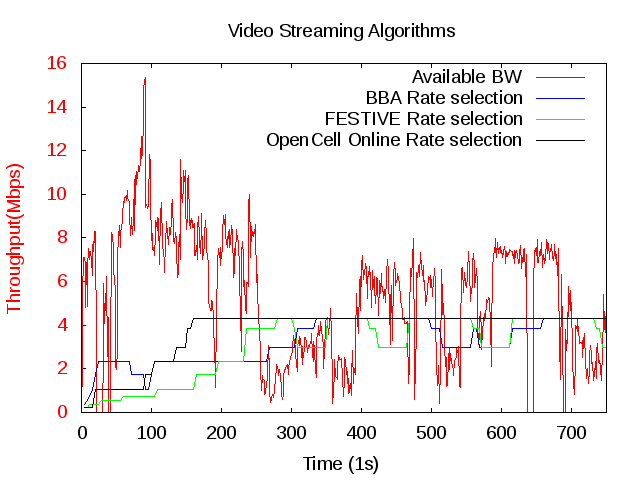
\includegraphics[width=\linewidth]{pictures/ATT.png}
 \caption{A sample trace from one major 4G network}
\end{figure}

\begin{table}[t]

\begin{tabular} {|c |c |c |c |}
\hline
\textbf{ Improvement} &\textbf{Quality} &\textbf{Stability} & \textbf{Interruption}\\ \hline
BBA(3G)  & 1.09x& 2.78x& 1x \\ \hline
FESTIVE(3G)    & 1.34x & 1.26x&5.5x\\ \hline
BBA(4G) & 1.16x& 2.1x& N/A \\ \hline
FESTIVE(4G) & 1.13x& 3.6x& N/A \\ \hline
\end{tabular}
\centering
\caption{Improvement with oracle estimator} \label{cap:table}
\end{table}


\subsection{Oracle Estimator}\label{sub:oracle}
In this section, the algorithm is using an "oracle" estimator, to show the space of improvement.

\emph{Key metrics improvement:} we measure three different metrics: quality (play efficiency), stability and interrupts. Play efficiency measures during the play session, the video downloaded and played vs available bandwidth. Stability measures the number of bit rate switches and interrupts measures the occurrence of interruption. Our algorithm outperforms the other two algorithms in all traces in terms of all three metrics, and the summary is in \autoref{cap:table}.

%\emph{Key metrics improvement:} we measure four different metrics: quality (play efficiency), stability and interrupts. Link utilization measures the total download vs available bandwidth, and the value is one if the link is constantly saturated. Play efficiency measures during the play session, the video downloaded and played vs available bandwidth, in the case without prefetched chunks, download utilization and play efficiency are equal. Stability measures the number of bit rate switches and interrupts measures the occurrence of interruption. Our algorithm outperforms the other two algorithms in all traces in terms of all four metrics, and the summary is in \autoref{cap:table}.

\emph{Prefetched buffer size}: we also compare the prefetched buffer size between BBA and our approach. FESTIVE is not client video buffer based solution and only adds randomized scheduling if it reaches a certain buffer level, we extend that buffer level to $z=240s$ download and see no difference in terms of its efficiency, stability or interruption, but we observe a little higher link utilization. Comparing BBA, we have reduced buffer size significantly by 20-30 seconds if we set $z=240$. We also notice no difference if we set $z=150$ in our new algorithm, however BBA suffers a higher oscillation in 4G traces. 


\emph{Comparison with Theoretical Max}: for a formulation in \autoref{subsec:offline}, we use IBM CPLEX to solve the mixed integer problem. We again replayed the 16 traces and the result shows that our approach can achieve 78.5\% close to the efficiency upper bound. In our offline algorithm one 3G trace has no feasible solution, and the reason is from the zero-interruption constraint, which also justifies the inevitability of interruption occurred in online algorithms. 

%\emph{Comparison with Modified FESTIVE}\Note{Not done yet!}: to show the performance gain is from both the novel algorithm and exposed extra KPIs, we also modified FESTIVE: we feed FESTIVE with a future bandwidth instead of using its harmonic mean estimation. 


\begin{table}[t]

\begin{tabular} {|c |c |c |c |}
\hline
 Improvement &Quality &Stability & Interruption\\ \hline
BBA(3G)  & 1.16x&1.6x &\textcolor{red}{0.9x} \\ \hline
FESTIVE(3G)& 1.40x &\textcolor{red}{0.86x}& 5x\\ \hline
BBA(4G) & 1.17x& 1.9x& N/A \\ \hline
FESTIVE(4G) & 1.14x& 3.4x& N/A \\ \hline
\end{tabular}
\centering
\caption{Improvement with noisy estimator} \label{cap:table2}
\end{table}

\subsection{Noisy Estimator}\label{sub:noisy}
We use a synthetic estimator for prediction and show that when the prediction is roughly accurate with a certain degree of error rate, our algorithm is robust to achieve a close-to-optimal performance. The key criterion for a good estimator is to have low error rate at each step and low to medium cumulative error rate over history. 

\emph{Noisy estimator}: we use a synthetic estimator to conduct a sensitive study for the new algorithm. The synthetic estimator makes prediction with a random factor in a N(1,0.2) distribution, means our prediction is $\geq$80\% accurate with 68\% chance, and $\geq 60\%$ accurate with 95\% chance. We run each syntheic estimator for 10 times for each trace and take the average. 

From \autoref{cap:table2} we can see that the quality is equal or even better, better quality is due to its higher sensitivity to high bandwidth estimations. However we lose some stability due to its unnecessary adjustments from inaccurate estimations, which leads to more frequent client play buffer changes. 

